\chapter{Pin Control Attack}
\label{chap:attack}

Before describing Pin Control Attack, a deeper analysis of the architecture of the target system is needed.
Note that, although this paper is focused on PLCs, the architecture described in the next section is still valid for almost any embedded system.
After having a proper knowledge of the underlying architecture, we can go deep into the description of the design of Pin Control Attack.
We consider the idea behind the attack, showing how it is able to evade the currently available detection mechanisms.
Next, we go further and describe some implementations of the attack, extending its applicability to a real Programmable Logic Controller.
Based on our architecture analysis and our tests, we can finally demonstrate that the attack is actually viable on real PLCs, even on a higher abstraction level.


\section{Embedded architecture}
\label{sec:embed_arch}

As briefly reported into \chap \ref{chap:intro}, PLCs use I/O interfaces to communicate with sensors and actuators, and in general with any external device.
Digging into their architecture, we know that PLCs are usually based on a so called System on Chip (SoC).
A SoC is basically an integrated circuit made of a microprocessor, a memory block and a set of peripheral controllers all enclosed together in the same chip substrate.
Thus, the SoC technology provides fully capable computers having both very small size and low power-consumption.
A SoC usually comes with a set of connections, also known as \emph{pins}, usually soldered to a printed circuit board to facilitate interconnection with external modules.
Many types of pins may be included in a SoC, having different purposes (power, clock, I/O, etc.).
An example of such a system is the Raspberry Pi board shown in \myfig{\ref{fig:raspberry}}, based on a Broadcom System on Chip.
\begin{figure}[h]
\centerline{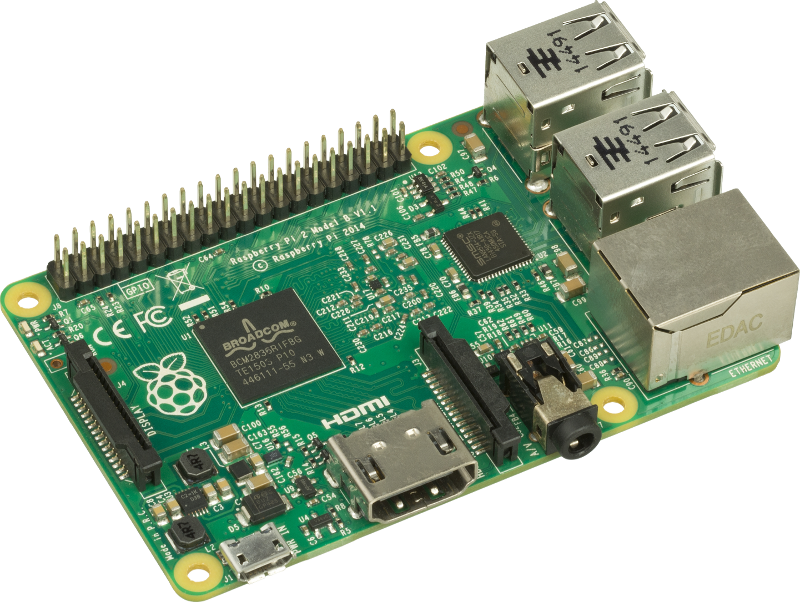
\includegraphics[width=0.56\textwidth]{res/raspberry}}
\caption{Raspberry Pi \cite{raspberry} with Broadcom System on Chip \label{fig:raspberry}}
\end{figure}
Actually almost all of the embedded systems use a SoC with similar boards, each one with its own size and configuration.

In order to accommodate many board implementations from different companies, each pin (or group of pins) of a SoC may have multiple configuration and operating modes.
The configuration of the pins is managed by the pin controller, a particular subsystem of a SoC.
Through a specific set of registers belonging to the pin controller, the system can configure the operating mode of the pins, such as their input or output mode.
These registers are typically accessible through a particular memory region called I/O memory. Such a kind of I/O access is known as \emph{Memory Mapped I/O}.

The features provided by a pin controller can be grouped into two main categories:
\begin{itemize}
	\item \itemname{pin configuration}: allows the system to change some electrical properties of the pins, such as direction, event detect, interrupt, etc.;
	\item \itemname{pin multiplexing}: each pin of the SoC may have many usages, also known as \emph{alternate functions}, depending on what is needed by the external board.
		The pin multiplexing feature enables the system to specify which type of function is needed on each pin.
\end{itemize}

As the I/O attack is a very low-level attack, it is necessary to dig further into the electrical world to know how these I/O interfaces work.


\subsection{SoC pins}
\label{sec:iopins}

I/O interfaces of a System on Chip provide a connection between internal modules and external electronic devices.
As shown in \myfig{\ref{fig:chips}}, they are physically visible from the outside of the chip package,
usually in the form of pins \subref{fig:pins} or soldering balls \subref{fig:balls}.

\begin{figure}[h]
\centering

\begin{subfigure}{.45\textwidth}
\centering
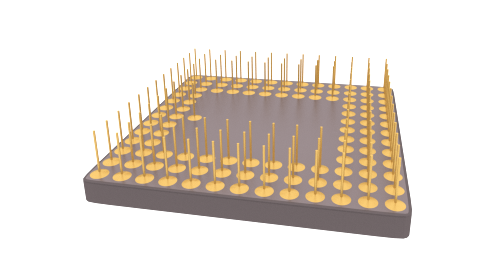
\includegraphics[width=\linewidth]{res/pins}
\caption{\label{fig:pins}}
\end{subfigure}
\begin{subfigure}{.45\textwidth}
\centering
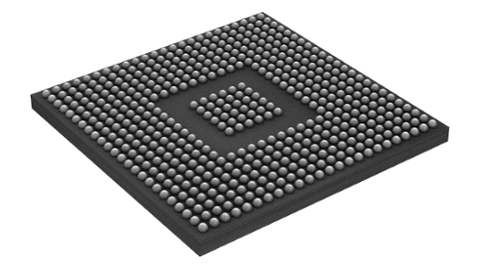
\includegraphics[width=\linewidth]{res/balls}
\caption{\label{fig:balls}}
\end{subfigure}

\caption{I/O connections packaged as \subref{fig:pins} Pin Grid Array and \subref{fig:balls} Ball Grid Array\label{fig:chips}}
\end{figure}

Internally they are connected to the silicon die through bonding wires, and are managed by a specific I/O circuit which may vary according to the specific chip.
Although there are many different implementations, almost all of the available SoCs have I/O ports with very similar functionalities.
For our purpose, we can describe them in an implementation-independent manner by using simplified generic schematics.


\subsubsection{Pin configuration}
\label{sec:pinconf}

The schematic depicted in \myfig{\ref{fig:pinconf}} helps us to discuss about the first set of features: pin configuration.
The operation mode described in this section is also known as General Purpose I/O (GPIO).

\begin{figure}[h]
\centerline{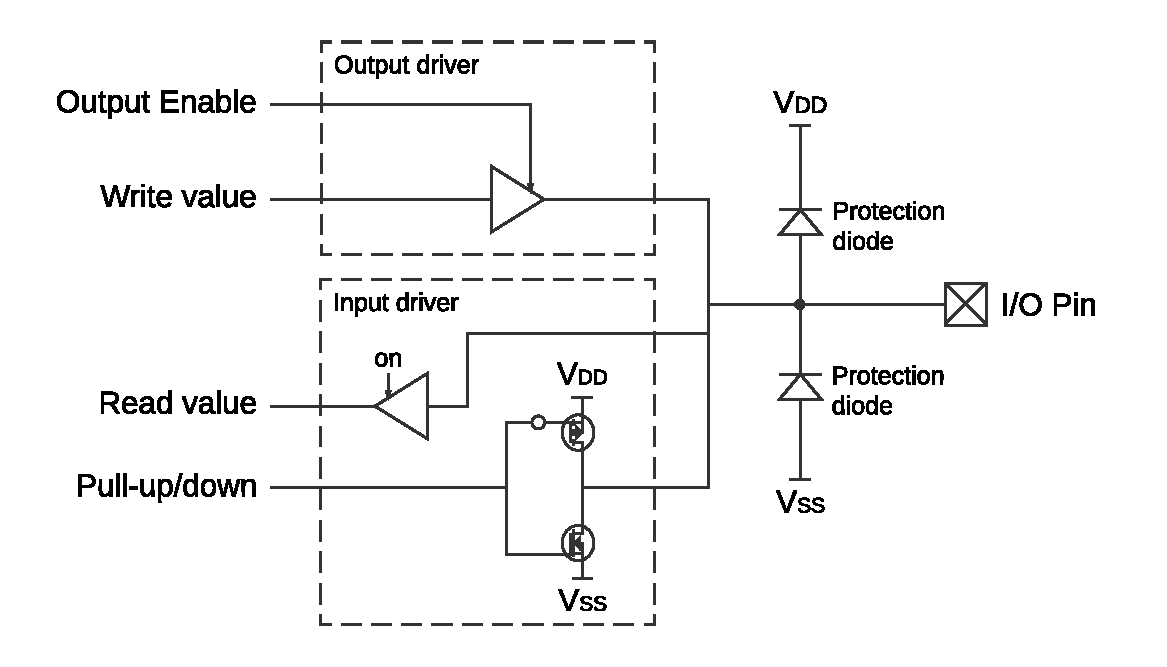
\includegraphics[width=0.8\textwidth]{res/pinconf}}
\caption{General Purpose I/O pin configuration circuit \label{fig:pinconf}}
\end{figure}

Apart from the protection diodes that serve as shield against input currents lower than $V_{SS}$ or higher than $V_{DD}$,
the circuit is divided into two different parts: one for output and one for input.
\begin{itemize}
	\item \itemname{Output driver}:
		The output module is basically a buffer controlled by an output enable signal.
		This signal controls the direction of the pin (input or output). If it is high, then the pin is in output mode
		and the value coming from a write operation goes through the buffer to the actual pin.
		If it is low, the pin is in input mode and the write signal is blocked, so it is not possible to change the external value of the pin from inside anymore.
	\item \itemname{Input driver}:
		The input driver has a similar buffer to read the value, usually having hysteresis capability which is useful for filtering unstable external values.
		Since the read buffer is always active, the input value is always available, even if the pin is currently working in output mode.
		The reason for this is merely physical: even if the external value was blocked by the buffer,
		one would always get a value by reading the input signal, because a value is nothing but an interpretation of the voltage level on a wire.
		When the pin is set as input, the pull-up/pull-down network enables the user to have a ``default'' value on the pin,
		namely a defined state maintained while the pin is not actively driven from outside. This feature is useful to avoid so called ``floating'' inputs.
\end{itemize}

For Pin Control Attack, what is more interesting about the circuit in \myfig{\ref{fig:pinconf}} are the following two properties:
\begin{itemize}
	\item there is no checking about the input state, so it is possible to perform a read even when the pin is in output mode;
	\item vice versa, it is not possible to write to a pin which has been configured as output.
\end{itemize}

Furthermore, it is also possible to drive the pull-up/down network, factually disturbing the real value of the I/O pin in an unpredictable way.
Virtually, it is even possible to interfere with the pin value by means of external electromagnetic fields.
In these cases the effects strongly depends on the actual implementation of the printed circuit board as well as on the external components connected to the I/O pin.


\subsubsection{Pin multiplexing}

Inside the chip an I/O pin may be connected to more than one device, which can be selected depending on the application,
that is the way of soldering or wiring the package into an electronic board.
This SoC feature is known as pin multiplexing (also ball multiplexing, pad multiplexing, alternate functions).
Even though pin multiplexing is designed for hardware configuration, in almost all modern chips it is possible to change the function at run-time.

\begin{figure}[h]
\centerline{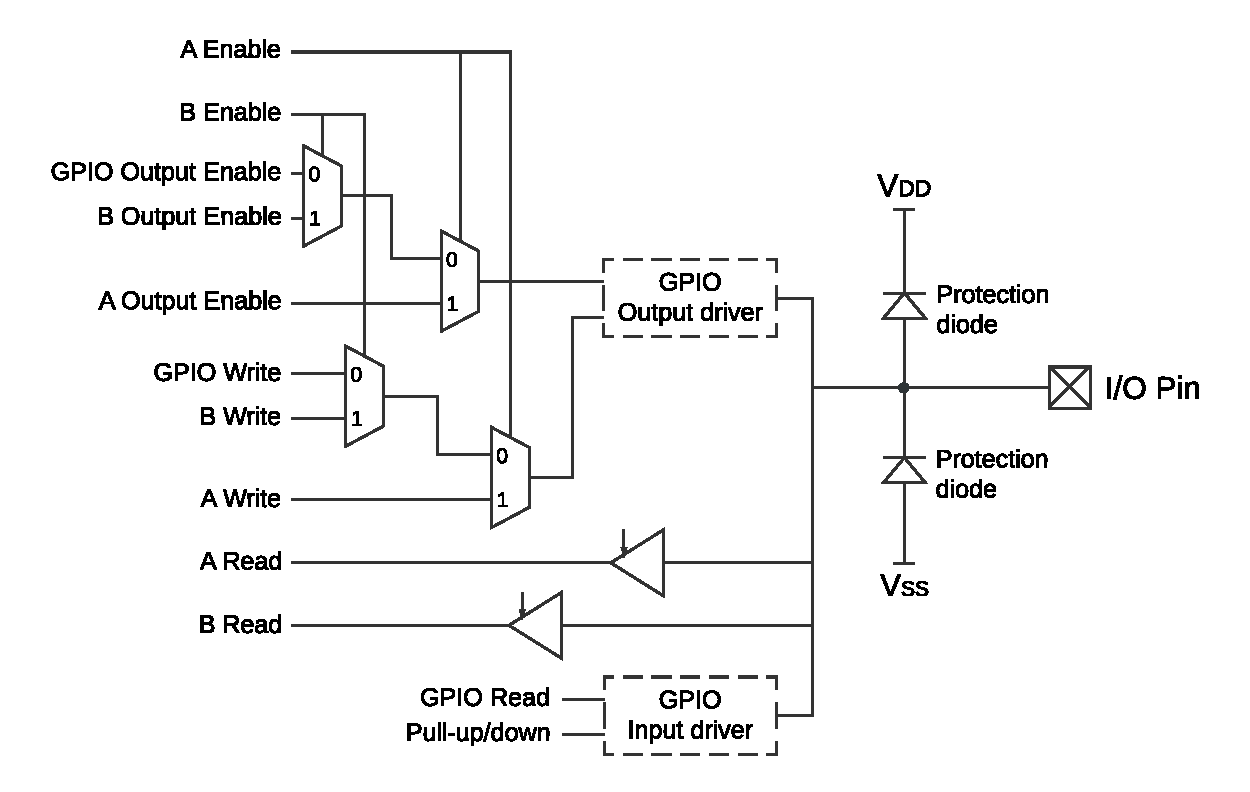
\includegraphics[width=0.8\textwidth]{res/pinmux}}
\caption{Generic I/O pin multiplexing circuit \label{fig:pinmux}}
\end{figure}

\myfig{\ref{fig:pinmux}}~ shows a possible hardware implementation of pin multiplexing.
The I/O pin in the figure is connected to two different peripherals inside the chip, namely A and B,
and it is also accessible through basic GPIO as described in \sec \ref{sec:pinconf} above.
The access to the GPIO output driver is regulated by two in cascade multiplexers for each signal of the module.
If the peripheral A is enabled, then the signals driven by A go through the multiplexers and can drive the actual value of the pin,
while GPIO and peripheral B output signals are blocked. Instead, if only peripheral B is enabled then only its signals are able to reach the I/O pin.
Note that in this last case the peripheral A should not be enabled, because A multiplexers have precedence against B ones.
Thus, the cascading of multiplexers actually implements a priority mechanism between peripherals A and B.
If neither A nor B are enabled, then no alternate function is active for the I/O pin and it could be driven by GPIO signals.
Each peripheral may also have its own dedicated input line, to get values from the I/O port in the same way as GPIO does.

For our purpose, at least two interesting properties can be inferred from pin multiplexing schematic of \myfig{\ref{fig:pinmux}}:
\begin{itemize}
	\item it is possible to block output signals from peripherals by simply changing the multiplexing configuration;
	\item the GPIO value can be read at any time, independently from the current multiplexing state of the output.
\end{itemize}


\subsection{PLC architecture}

As introduced in \chap \ref{chap:intro}, Programmable Logic Controllers are a particular kind of embedded systems,
designed to work into harsh environments and to control a physical process, typically an industrial or other critical processes.
In this section we examine the hardware and the software architecture of a PLC. This analysis will be needed later to better explain
the threat model and the implementation of Pin Control Attack.


\subsubsection{Hardware architecture}

Since it is built for working into a rough environment, the internal hardware of a PLC is shielded and not directly visible as the Raspberry Pi one.
\myfig{\ref{fig:wagoplc}} shows an example of a basic PLC, provided by Wago. This model will be later used for our tests.
Note that, although we provide this specific example, the basic concepts described here are still valid for most of the PLC on the market, unless otherwise specified.

\begin{figure}[h]
\centerline{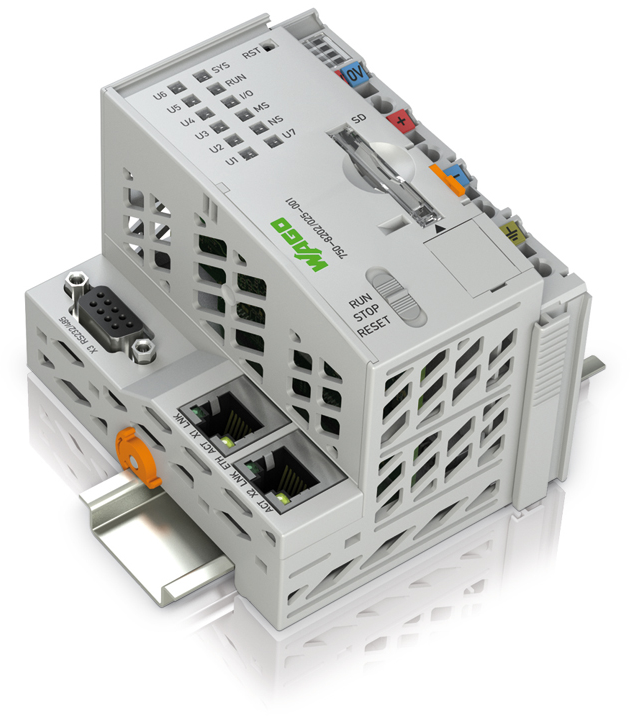
\includegraphics[width=0.5\textwidth]{res/wagoplc}}
\caption{PFC200 Programmable Logic Controller from Wago \label{fig:wagoplc}}
\end{figure}

Internally, the PLC has a System on Chip whose architecture is substantially equivalent to the one discussed in the above sections.
Therefore, the same concepts are applicable to PLCs as well.
Anyway, from our analysis we found that their architecture could be a bit more complicated with respect to a plain SoC.
Since the environment in which PLCs work may greatly differ case by case, they are designed to be as versatile as possible.
Vendors know that their PLC could be deployed in many different physical processes, possibly having completely diverse sensors and actuators to interact with.
Clearly, it is unreasonable to put every possible I/O interface on the same SoC. For this reason, most of the available PLCs comes with the possibility
of connecting a certain number of external components called \emph{I/O modules}. Each I/O module contains its own embedded SoC,
responsible for a specific subset of I/O interfaces (\eg digital input/output, analog input/output, pulse-width modulation, communication, etc.).
This hardware architecture is summarised in \myfig{\ref{fig:plc_arch}}.

\begin{figure}[h]
\centerline{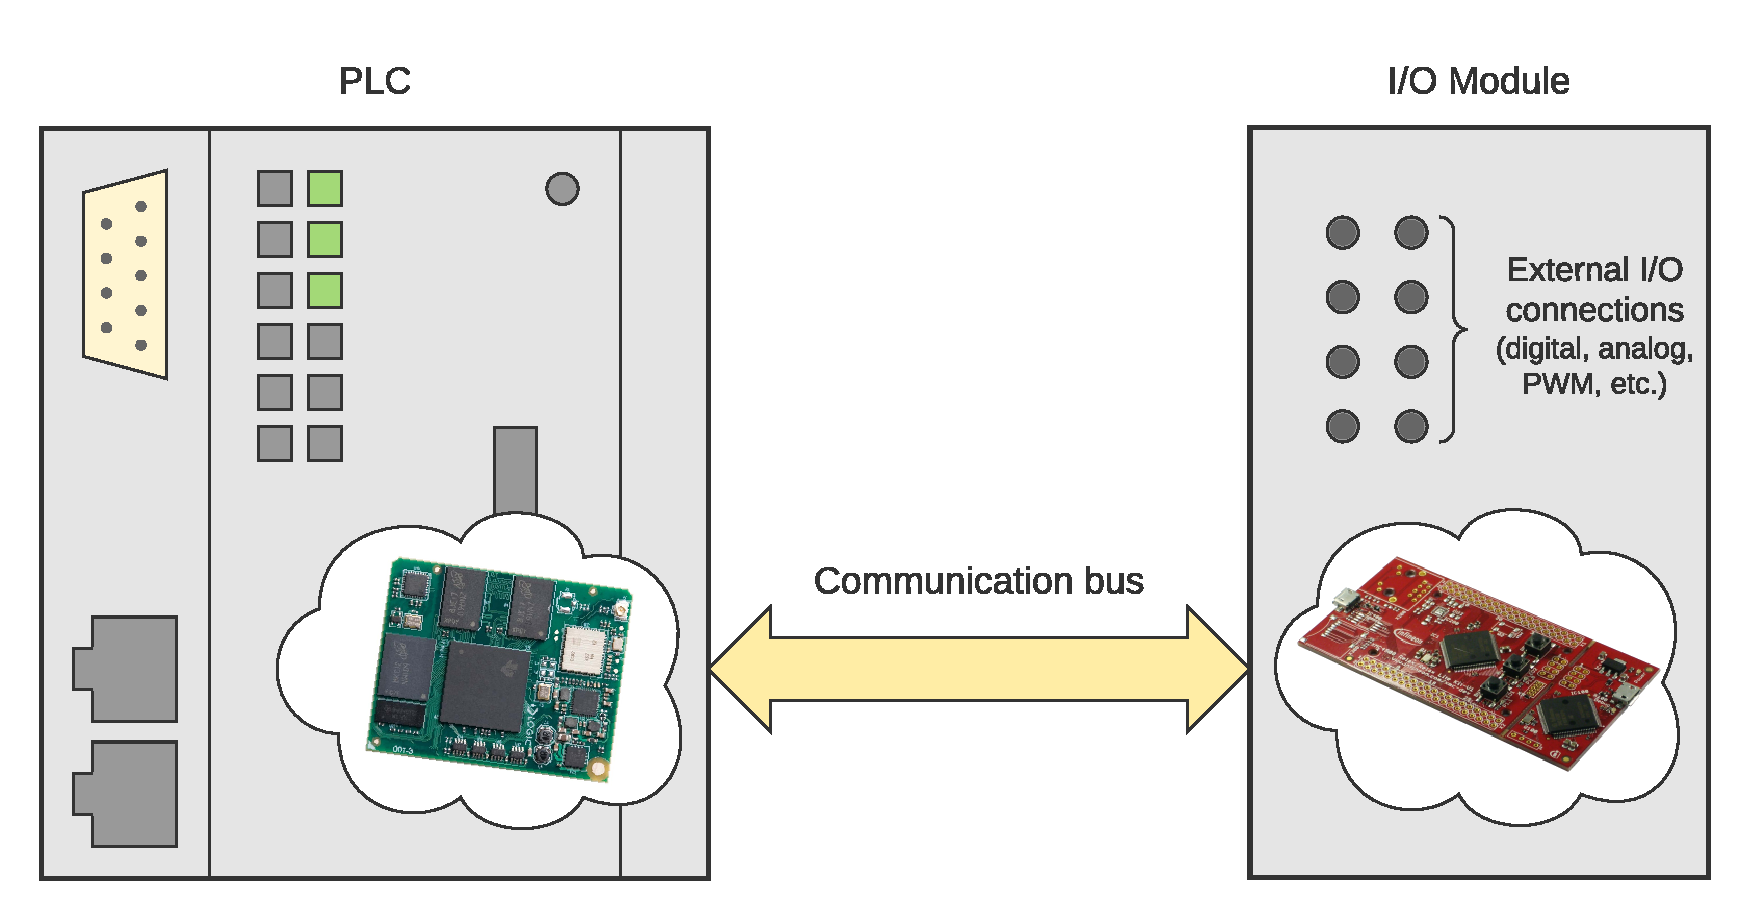
\includegraphics[width=0.8\textwidth]{res/plc_arch}}
\caption{PLC hardware architecture \label{fig:plc_arch}}
\end{figure}

The main portion of the PLC communicates with the I/O modules via a system bus, which is, in turn, connected to the I/O interfaces of the PLC.
This architecture with I/O modules adds one level of indirection between the targeted PLC and the external world, since there is another SoC in the middle.
Anyway, the same concepts of Pin Control Attack can be applied to such an architecture as well. It is sufficient to consider that the I/O interface of the PLC,
connected to the internal bus, is now the new direct target of our attack, while the final I/O becomes an indirect target. As we demonstrate in \sec \ref{sec:attack_plc},
by tampering with the I/O related to the communication bus it is possible to achieve equivalent results, proving that Pin Control Attack is still applicable on real PLCs.


\subsubsection{Software architecture}

The PLC typically comes with a real-time operating system (\eg Linux with RT-preempt patch, VxWorks etc.), because of the time requirements imposed by its main task.
Above the operating system, a software called \emph{PLC runtime} is responsible for managing the execution state of the control process and regulating the access to the PLC.
Through the runtime, the industrial operator can connect its terminal to the PLC and upload the desired control program, the \emph{logic}.
The PLC logic is the application code responsible for the control of the physical process, dealing with input and output interfaces.
As shown in \myfig{\ref{fig:plc_swarch}}, this architecture can be divided into three layers, laying one above the other.

\begin{itemize}
	\item \itemname{Firmware}: the lowest layer, which basically corresponds to the operating system kernel. Although they are typically two distinct parts,
		here we consider the bootloader also as ``part'' of the firmware, because in this context their separation is irrelevant.
	\item \itemname{Runtime}: a software which is part of the application layer above the firmware, and it is started by the operating system itself.
	\item \itemname{Logic}: the control program running within the runtime environment. Its execution is started and stopped by the runtime,
		and its code is dynamic: it may change whenever the industrial operator decides to upload a new control program to the PLC.
\end{itemize}

\begin{figure}[h]
\centerline{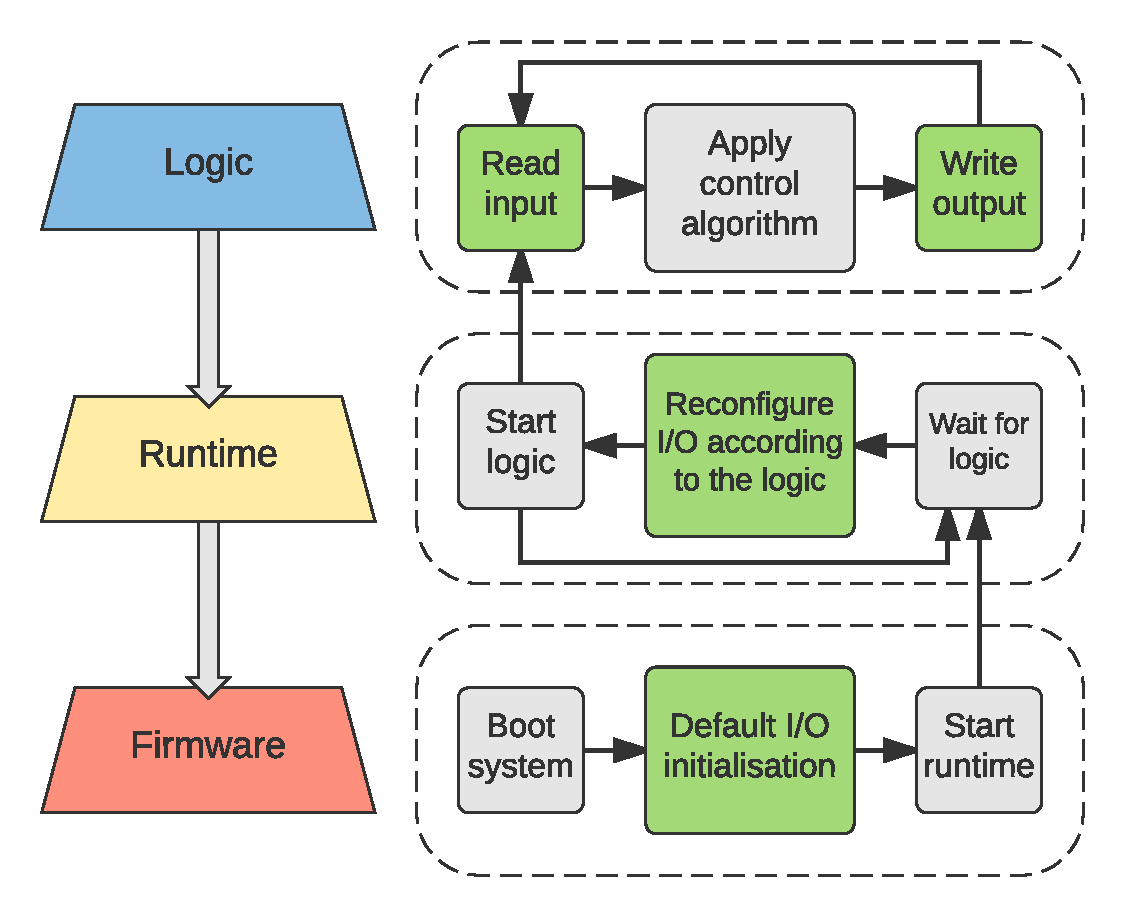
\includegraphics[width=0.7\textwidth]{res/plc_swarch}}
\caption{PLC software architecture \label{fig:plc_swarch}}
\end{figure}

\myfig{\ref{fig:plc_swarch}} also summarises the execution flow of each layer, from bottom to top, highlighting (in green) the tasks directly related with the I/O.

When the firmware is loaded into memory and the system is booting, one of the early operation performed is the I/O initialisation.
In this phase, the drivers loaded within the kernel start to configure their own I/O registers with their default values.
Depending on the implementation, this may be the configuration desired by the final application, or not. That is, the I/O configuration may be changed later in time.
After the I/O has been initialised, the firmware loads the main application needed by the controller: the runtime.

The PLC runtime waits for a logic to be uploaded into the PLC from a terminal connected via the network interface.
The execution flow reported in \myfig{\ref{fig:plc_swarch}} is a general process, including the case when a PLC is started for the first time.
If a PLC is already in production, it is rarely restarted. However, when a reboot is needed (\eg for firmware update),
it may be configured to persistently save the current logic into a non-volatile memory and restore it after reboot.
In this case the wait step in \myfig{\ref{fig:plc_swarch}} can be simply skipped.

When a logic is available, from network or from disk, the PLC runtime analyses its content.
The I/O configuration expected by a specific logic is bundled with the logic itself, because it is decided by the operator who has knowledge of the physical process
and knows how sensors and actuators are connected to the PLC I/O ports. With respect to the hardware architecture shown in \myfig{\ref{fig:plc_arch}},
a change in the input/output required by the operator is actually reflected into a configuration change of the external I/O modules.
Whether this process involves a change in the I/O configuration of the PLC itself depends on the implementation and on the modification extend
(\eg if a new I/O module has been attached, this will probably require a change in the communication protocol and so on the I/O interface of the PLC).
After the new I/O configuration has been applied, the logic can be executed. From an operating system point of view, the logic is running in the same context of the PLC runtime.

As briefly discussed in \chap \ref{chap:intro}, the PLC logic executes the main \emph{scan cycle}. For each iteration, it reads from inputs, executes the control algorithm,
and writes to outputs. The control algorithm has been programmed by the industrial operator, and loaded through the interface provided by the PLC runtime.
When the logic is running, input and output pins have already been configured by the runtime, and the logic assumes that the I/O configuration does not change during its execution.
Both the logic and the runtime interacts with the I/O, but in different ways. The runtime deals with I/O configuration registers, while the logic performs read/write operations
related to I/O values. Both kind of interactions, anyway, require the same privileges, which will be later leveraged by Pin Control Attack.


\section{Attack Design}

Given the properties discussed in \sec \ref{sec:embed_arch}, it is possible to misuse the registers used to configure I/O peripherals,
and that is what Pin Control Attack does. This can happen at run-time, during the execution of the controller on a real process,
without any reaction from the PLC runtime or the operating system, thus remaining completely stealth.

We can argue that Pin Control Attack is actually applicable on any System on Chip having the
architecture described in \sec \ref{sec:embed_arch}. However, PLCs represent a particularly interesting target among all the embedded systems based on SoC.
PLCs leverage the interfaces of a SoC to interact with sensors and actuators, having direct effects on our physical world.
Therefore, if the I/O of a PLC is compromised, this constitutes a much more significant security and safety risk with respect to other
non-critical embedded system. For this reason, PLCs represent one of the most attractive targets for Pin Control Attack.

In this section we focus on the design of I/O attack. First, we summarise the host-based detection mechanisms taken into account
during the attack design and the techniques used to evade them. Second, we analyse the attack itself in more detail.
The goal of this chapter is to help us having a better understanding of the attack, and to provide a detailed threat model on which our defense design will be based on.

Pin Control Attack has been designed to be different from previous attack techniques, and to circumvent the off-the-shelf host-based detection systems.
The authors of I/O attack have identified two main defensive mechanisms whose properties makes them more easily applicable to PLCs.
Here we want to generalise and consider them in our threat model, clarifying how and when Pin Control Attack becomes applicable and interesting for attackers.
We also show how these defenses are circumvented by Pin Control Attack, and describe the available attack techniques.
We do not repeat here the detailed description made in \cite{ghostplc}. We only want to have basic concepts definition,
in order to be able to focus on our further analysis and implementation of the attack.


\subsection{Defense analysis}
\label{sec:def_analysis}

At this point, one could ask why descending to the lowest level possible to conduct an attack, when a lot of easier techniques (\eg function hooking) may achieve equivalent results.
The point here is that many producers of embedded systems and PLCs already started to move towards a more security-aware production.
As considered in \cite{ghostplc}, in order to be applicable to PLCs, a defensive mechanism should have at least the following properties:
\begin{itemize}
	\item low CPU overhead: CPU resources are limited in embedded systems such as PLCs, which typically have hard real-time constraints;
	\item designed to run on an operating system: almost all of the modern PLCs have a real-time OS running on it;
	\item no hardware modification required: many solutions are hardware-based \cite{trustlite,hardware-ibmac,ocfmm,fine-grained,bb-cfi}, making them not easily applicable;
	\item no virtualisation required: the majority of embedded systems, like PLCs, does not support virtualisation;
		thus solutions like \cite{hypervisor-control} are less attractive.
\end{itemize}

Given these considerations, we can list some of the applicable defenses:
\begin{itemize}
	\item \itemname{SEM}: the Symbiote detection system described in \cite{symbiotes}, which protects the kernel from code modification attacks;
	\item \itemname{Autoscopy Jr.}: the lightweight intrusion detection system proposed in \cite{autoscopy}, effective against control flow manipulation inside the kernel.
\end{itemize}

The above detection systems still have some shortcomings, leveraged by Pin Control Attack.
First, they are based on a comparison with golden references (the symbiotes and the TLL, respectively) taken from a subset of the entire kernel space.
If the attacker is able to find a portion of the kernel space which has not been considered by the detection system, then it can be circumvented.
For example, Autoscopy Jr. can be bypassed if the attacker is able to craft a duplicate of the kernel functions it needs.
If a duplicate function is used instead of the original version, Autoscopy Jr. does not throw an alert, because this function is not listed in the TLL at all.
Second, the references used by both defenses are \emph{static}, which means that they are based on previous analysis of the immutable (static) portion of the system.
Thus, an attacker could still use dynamic memory, whose content changes during run-time, to conduct its own attack.
In the case of SEM, only static code regions (which are immutable) are taken into account, so any malware placed in dynamic memory will not be detected.
Autoscopy Jr., instead, considers the function pointers used inside the kernel, including the ones inside the System Call Table and other similar tables.
Therefore, it is able to detect only \emph{data hooks} but not \emph{code hooks}, that is, any direct code modification (\eg of the kernel text) is still possible.

Anyway, these two defenses may be used in combination, thus providing a host-based IDS able to detect both code and data hooks.
Even if they are deployed together, however, attacks through dynamic memory and without function hooking are still possible,
since monitoring dynamic memory is a far more complex issue. One of the implementations of Pin Control Attack (see \sec \ref{sec:attack_impl})
leverages exactly the kernel dynamic memory to reach its purpose.

Host-based detection mechanisms like the ones discussed above will likely be deployed into many commercial products within the next years \cite{symbiote_web, autoscopy_web},
raising the bar for attackers. Therefore, Pin Control Attack will become more and more interesting as long as classical techniques (\eg function hooking) are overcome.


\subsection{Threat model}

In our work, we assume that the system is protected at least by the HIDSs described in \sec \ref{sec:def_analysis}, or equivalent.
Hence, we assume that the attacker cannot tamper with operating system (kernel) functions and data structures, but it can still use dynamic memory to insert its malicious code
and tamper with the I/O configuration. The attacker can also write its own version of kernel functions if needed, and call them separately in order to avoid HIDSs.
This approach, anyway, requires very high effort and would really be the last option for an attacker.

The attacker, depending on the attack implementation, may need different running privileges on the target system to execute Pin Control Attack.
Generally speaking, the minimum privilege required is the privilege level of the PLC runtime, which has access to the I/O configuration registers.
As already discussed in \cite{ghostplc}, many ICS-CERT advisories have shown that PLCs have vulnerabilities that could lead to malicious code execution
\cite{plc-network,abb-codesys,codesys-server,schneider-bof,rockwell-vuln,rockwell-vuln2}, and they may affect PLC runtime software as well.
Thus, obtaining the same PLC runtime privilege level is feasible on real systems.

As in \cite{ghostplc}, we assume that the attacker knows both the physical process controlled by the target system and the mapping
between I/O configuration and external sensors and actuators. The former is typically known by the attacker, which has reasonably studied its target before conducting the attack.
This is confirmed by Stuxnet \cite{stuxnet}, where attackers had very deep knowledge of target system and physical process.
The latter is given by a knowledge of the PLC logic, which, as said, already comes with the mapping between I/O interfaces and control variables used by the logic.
Furthermore, the research presented in \cite{dynamic-payload,sabot} shows that it is possible to infer the structure of the devices connected to the PLC and used by the logic,
factually lowering the bar for attackers which do not need an a priori knowledge of the I/O mapping anymore.


\subsection{Pin Control Attack}

Based on the previous assumptions, Abbasi et al. \cite{ghostplc} crafted Pin Control Attack, which is capable of manipulating the physical process
controlled by a PLC without requiring any firmware or logic modification.
The idea of Pin Control Attack is that the attacker operates at the lowest level possible, targeting the interaction
between the firmware and the I/O, as shown in \myfig{\ref{fig:target}}. For this reason the attack is also known as I/O attack.
Despite its crucial function in embedded systems, I/O hardware architecture and I/O drivers are currently designed
without taking into account any concept of security, assuming that I/O is reliable. Unfortunately, given the properties inferred in \sec \ref{sec:embed_arch}
from a generic hardware architecture, this is often not the case.

\begin{figure}[h]
\centerline{\includegraphics[page=6,viewport=50 620 300 750,clip]{res/ghostplc}}
\caption{Pin Control Attack target, from \cite{ghostplc} \label{fig:target}}
\end{figure}

As described in \cite{ghostplc}, Pin Control Attack is designed to evade off-the-shelf HIDSs presented in \sec \ref{sec:def_analysis}.
In particular, it leverages kernel dynamic memory (in one implementation variant) or it uses a simple user code (in a second variant).
Both variants are able to circumvent the above detection mechanisms.

The authors of \cite{ghostplc} have found at least two different attack vectors for Pin Control Attack: \emph{Pin Configuration} and \emph{Pin Multiplexing}.
Both kind of attacks leverage the SoC properties described in \sec \ref{sec:embed_arch}.
The attack is performed by misusing the control registers used to program the I/O peripherals, writing malicious values into them.
If the attack targets I/O configuration registers, it is a Pin Configuration Attack, otherwise, if the targeted registers are related to the multiplexing state of the pins,
then it is a Pin Multiplexing attack. In some architectures, I/O configuration and multiplexing is achieved by using the same set of registers
(\eg different values written on the same register may have different purposes).

Moreover, we imagine that many other attack possibilities may exist. An attacker can tamper with the I/O configuration in many other ways depending on the
specific I/O peripheral and on its features (\eg event detect, interrupts, clock signals, etc.), and the effects of the attack are unpredictable.
If the attacker can analyse the reference manual of the target SoC (mostly publicly available) and it has enough competence and time,
the only limit to Pin Control Attack becomes fantasy.
To give an idea of what such an attack can do, imagine a simple SoC pin which can be multiplexed between a memory controller and a PWM controller.
If this pin is actually connected to an external memory, thus multiplexed as memory controller, a Pin Multiplexing attack can lead to dangerous signals
sent from a PWM controller to a memory module, which may burn the memory.

On the other side, from our analysis on a real PLC, we found that another attack vector is viable at a different abstraction level than hardware configuration.
Commonly, the I/O peripherals are used through operating system drivers, which in turn are used from user space applications like the PLC runtime.
As we show in \sec \ref{sec:attack_plc}, an attacker can target these drivers, or even these applications, to obtain equivalent effects without dealing with
the underlying hardware and/or I/O registers directly.


\section{Attack Implementation}
\label{sec:attack_impl}

TODO Implementation.


\subsection{Raspberry Pi}

TODO Raspberry Pi implementation.


\subsection{PLC}
\label{sec:attack_plc}

TODO PLC implementation.
